\documentclass[11pt]{article}
\usepackage{fullpage}
\usepackage{amsfonts}
\usepackage{graphics}

\def\eq1{y = \frac{3x}{x^3 + 88x + 90}}
\begin{document}
	\title{Tutorial 6}
	\author{Prashant Singh}
	\date{\today}
	\maketitle
	
	The set of natural numbers is denoted by $\mathbb{N}$.
	
	The set of integer numbers is denoted by $\mathbb{Z}$.
	
	The set of real numbers is denoted by $\mathbb{R}$.
	
	Grapg $\eq1$
	
	Draw the asymptote of $\eq1$
	
	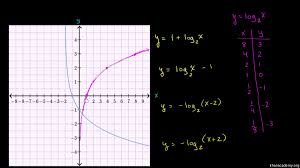
\includegraphics[scale=0.75]{index.jpeg}
\end{document}